%%%%%%%%%%%%%%%%%%%%%%%%%%%%%%%%%%%%%%%%%
% Thin Sectioned Essay
% LaTeX Template
% Version 1.0 (3/8/13)
%
% This template has been downloaded from:
% http://www.LaTeXTemplates.com
%
% Original Author:
% Nicolas Diaz (nsdiaz@uc.cl) with extensive modifications by:
% Vel (vel@latextemplates.com)
%
% License:
% CC BY-NC-SA 3.0 (http://creativecommons.org/licenses/by-nc-sa/3.0/)
%
%%%%%%%%%%%%%%%%%%%%%%%%%%%%%%%%%%%%%%%%%

%----------------------------------------------------------------------------------------
%	PACKAGES AND OTHER DOCUMENT CONFIGURATIONS
%----------------------------------------------------------------------------------------

\documentclass[letterpaper,10pt]{article} % Font size (can be 10pt, 11pt or 12pt) and paper size (remove a4paper for US letter paper)
\usepackage{geometry}
\geometry{paperwidth=4in,margin=.1in,paperheight=35in}
\usepackage[protrusion=true,expansion=true]{microtype} % Better typography
\usepackage{graphicx} % Required for including pictures
\usepackage{caption}
\usepackage{subcaption}
\usepackage{wrapfig} % Allows in-line images
\usepackage{amsmath,amsthm}
\usepackage{thmtools}
\usepackage{xfrac}
\usepackage{mathpazo} % Use the Palatino font
\usepackage[T1]{fontenc} % Required for accented characters
\linespread{1.05} % Change line spacing here, Palatino benefits from a slight increase by default

\makeatletter
\newcommand{\pipe}{\;\middle\vert\;}
\newcommand{\condp}[2]{\Pr\left( #1 \pipe #2 \right)}
\newcommand{\pr}[1]{\Pr\left( #1 \right)}
\newcommand{\condpe}[2]{\frac{\pr{#1,#2}}{\pr{#2}}}
\newcommand{\condpb}[2]{\frac{\condp{#2}{#1}\pr{#1}}{\pr{#2}}}
\newcommand{\norm}[1]{\left|#1\right|}
\DeclareMathOperator*{\argmin}{arg\,min}
\DeclareMathOperator*{\argmax}{arg\,max}
\newcommand{\half}{\frac{1}{2}}
%theorem styling
\declaretheorem{theorem} 
\declaretheoremstyle[%
spaceabove=-6pt,%
spacebelow=6pt,%
headfont=\normalfont\itshape,%
postheadspace=1em,%
qed=\qedsymbol,%
headpunct={}
]{mystyle} 
\declaretheorem[name={},style=mystyle,unnumbered,
]{Proof}

\newcommand{\prove}[1]{
\begin{Proof}
\begin{align*}
#1
\end{align*}
\end{Proof}
}

\newcommand{\lm}{\lambda}
\newcommand{\LML}[2]{\lm #1 + (1-\lm) #2}
\newcommand{\difrac}[2]{\frac{\delta #1}{\delta #2}}
\renewcommand{\@listI}{\itemsep=0pt} % Reduce the space between items in the itemize and enumerate environments and the bibliography

\renewcommand{\maketitle}{ % Customize the title - do not edit title and author name here, see the TITLE block below
\begin{flushright} % Right align
{\LARGE\@title} % Increase the font size of the title

{\large\@author} % Author name
\\\@date % Date

\end{flushright}
}

%----------------------------------------------------------------------------------------
%	TITLE
%----------------------------------------------------------------------------------------

\title{\textbf{Assignment 3}\\ % Title
Machine Learning 10-701} % Subtitle

\author{\textsc{Arjun Menon} % Author
\\{\textit{Carnegie Mellon University}}} % Institution

%----------------------------------------------------------------------------------------

\begin{document}

\maketitle % Print the title section

\section{Probability Inequalities}

\subsection{1.1}

\subsubsection*{(a)}

Let $p$ be the probability the coin flip comes up heads.

\begin{align*}
\pr{\bar{X}_n \geq a} = \pr{\bar{X}_n \geq \sfrac{1}{2}} &\leq \frac{E[\bar{X}_n]}{\sfrac{1}{2}} \\
&= 2 E\left[ \frac{1}{n} \sum^n_{i=1} X_i \right] \\
&= \frac{2}{n} \sum^n_{i=1} E\left[ X_i \right] \\
&= \frac{2}{n} \sum^n_{i=1} (p \times 1 + (1-p) \times 0) \\
&= \frac{2}{n} n p \\
\pr{\bar{X}_n \geq \sfrac{1}{2}} &\leq 2p \\
\end{align*}

Thus for a biased-heads coin ($ p>\sfrac{1}{2} $) then the Probability is unbounded upperbound.

\subsubsection*{(b)}

Given Chebyshev's inequality,

\begin{align*}
\pr{\left|\bar{X}_n - \mu\right| \geq k} &\leq \frac{\sigma^2}{k^2}\\
\end{align*}

We use the fact that,

\begin{align*}
E\left[ \bar{X}_n \right] = \mu = p\\
\end{align*}

and,

\begin{align*}
\mathrm{Var}\left[ \bar{X}_n \right] = \sigma^2 &= \frac{1}{n^2} \sum_{i=1}^n\mathrm{Var}\left[X_i \right] \\
&= \frac{np(1-p)}{n^2} \\
&= \frac{p(1-p)}{n} \\
\end{align*}

and for our choice of $k$, we pick such that

\begin{align*}
\bar{X}_n &\geq \sfrac{1}{2} \\
\bar{X}_n - \mu &= \sfrac{1}{2} - \mu \\
\implies k &= \sfrac{1}{2}-\mu \\
\end{align*}

Therefore only when $p < \sfrac{1}{2}$, then we can apply Chebyshev's inequality,

\begin{align*}
\pr{\left|\bar{X}_n - \mu \right| \geq \sfrac{1}{2}-\mu} &\leq \frac{(\frac{p(1-p)}{n})^2}{(\sfrac{1}{2}-\mu)^2}\\
\pr{\left|\bar{X}_n - p\right| \geq \sfrac{1}{2}-p} &\leq \frac{p(1-p)}{n(\sfrac{1}{2}-p)^2} \\
\end{align*}

which holds for only for $p<\sfrac{1}{2}$.

\subsubsection*{(c)}

For Heoffding's inequality, 

\begin{align*}
\pr{\left|\bar{X}_n - \mu \right| \geq \epsilon} \leq 2e^{-2n\epsilon^2 /(b-a)^2}\\
\end{align*}

which for a biased coin, we use the result above that $\epsilon = \sfrac{1}{2} - p$ thus obtaining

\begin{align*}
\pr{\left|\bar{X}_n - \mu \right| \geq \epsilon} \leq 2e^{-2n(\sfrac{1}{2} - p)^2}\\
\end{align*}

\subsubsection*{(d)}

Initially Markov is tightest, but then Chebyshev is tightest from the range of $n=~5$ to $n=20$, after which Hoeffding is the tightest bound.

\begin{figure}[h]
\centering
\begin{subfigure}[b]{\textwidth}
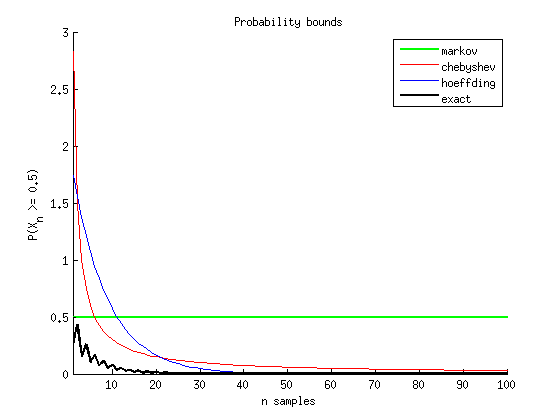
\includegraphics[width=\textwidth]{figs/p1de}
\caption{Probability bounds: Markov, Chebyshev, and Hoeffding}
\label{fig:p1de}
\end{subfigure}%

\begin{subfigure}[b]{\textwidth}
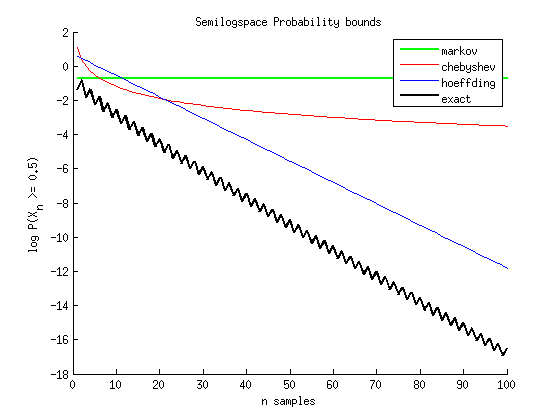
\includegraphics[width=\textwidth]{figs/p1f}
\caption{Semilogspace probability bounds}
\label{fig:p1f}
\end{subfigure}

\begin{subfigure}[b]{\textwidth}
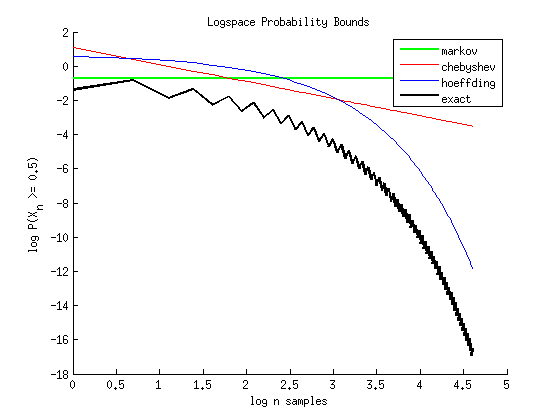
\includegraphics[width=\textwidth]{figs/p1g}
\caption{Logspace probability bounds}
\label{fig:p1g}
\end{subfigure}

\caption{}\label{fig:p1}
\end{figure}

\subsubsection*{(e)}

See Figure~\ref{fig:p1de}
\subsubsection*{(f)}
See Figure~\ref{fig:p1f}
\subsubsection*{(g)}
See Figure~\ref{fig:p1g}
\subsubsection*{(h)}
In original space, only the Markov bound is linear, since it is a constant with respect to the number of samples.

In semi-log space, the Markov and Hoeffding bounds are linear. Hoeffding is linear now because $n$ is in the exponent in the original bound. Therefore $n$ will vary with itself linearly.

In log-log space, the Markov and Chebyshev bounds are linear. Chebyshev is linear because $\log n$ varies with

\begin{align*}
\log ( \pr{\left|\bar{X}_n - p\right| \geq \sfrac{1}{2}-p} ) &\leq \log \left( \frac{p(1-p)}{n(\sfrac{1}{2}-p)^2} \right) \\
\log ( \pr{\left|\bar{X}_n - p\right| \geq \sfrac{1}{2}-p} ) &\leq -\log(n) + \log \left( \frac{p(1-p)}{(\sfrac{1}{2}-p)^2} \right) \\
\end{align*}

linearly.

%------------------------------------------------
%\bibliographystyle{unsrt}
%\bibliography{sample}

%----------------------------------------------------------------------------------------

\end{document}
